%% A Self-Contained Real-Time Detection Pipeline and an Operating-Point Replay
%% Protocol Applied to Turkish Broadband Stations.
%% Computers & Geosciences submission draft (v12), in the
%% journal's template (cas-sc.cls, cas-common.sty, cas-model2-names.bst, from
%% github.com/cageo/CAGEO_LaTeXTemplate, commit 965ebcc).
%%
%%   make            paper.pdf
%%
\documentclass[a4paper,fleqn]{cas-sc}

\usepackage[authoryear]{natbib}
\usepackage{graphicx}
\usepackage{amsmath}
\usepackage{booktabs}
\usepackage{makecell}
\usepackage{array}
\usepackage{setspace}
\usepackage[nomarkers,figuresonly]{endfloat}
\usepackage{lineno}
% The template's \cortext ends up printing its "[COR: Number]" trace on the
% first page in this build; send the trace to the log only.
\ExplSyntaxOn
\cs_set_protected:Npn \msg_term:n #1 { \iow_log:n {#1} }
\ExplSyntaxOff
% The template records the page count for its "Page X of N" footer before
% endfloat has output the figures at the end; record every shipped page's
% number instead, so that the last one wins.
\makeatletter
\AddToHook{shipout/before}{\immediate\write\@auxout{\string\csxdef{lastpage}{\thepage}}}
\makeatother
\linenumbers

\newcommand{\Mw}{$M_\mathrm{w}$}
\newcommand{\VP}{$V_\mathrm{P}$}
\newcommand{\VS}{$V_\mathrm{S}$}
\newcommand{\stalta}{STA/LTA}
\newcommand{\tablenote}[1]{\par\vspace{4pt}%
  \begin{minipage}{\linewidth}\footnotesize\textit{Note.} #1
\end{minipage}}
\newcolumntype{L}[1]{>{\raggedright\arraybackslash}p{#1}}

\begin{document}
\let\WriteBookmarks\relax
\def\floatpagepagefraction{1}
\def\textpagefraction{.001}
\shorttitle{A self-contained detection pipeline and an operating-point replay protocol}
\shortauthors{H.O. Bolat et al.}

\title [mode = title]{A Self-Contained Real-Time Detection Pipeline and an
Operating-Point Replay Protocol Applied to Turkish Broadband Stations}

\author[1]{H. O\u{g}uz Bolat}[orcid=0009-0000-8522-7746]
\cormark[1]
\ead{oguz.bolat@std.yildiz.edu.tr}
\credit{Conceptualization, Methodology, Software, Investigation, Formal analysis,
Data curation, Visualization, Writing -- original draft}

\author[2]{Sibel \c{C}imen}[orcid=0000-0003-3790-7362]
\credit{Writing -- review and editing}

\author[2]{B\"ulent Bolat}[orcid=0000-0002-2468-8618]
\credit{Writing -- review and editing, Supervision}

\author[2]{T\"ulay Y\i{}ld\i{}r\i{}m}[orcid=0000-0001-9993-5583]
\credit{Writing -- review and editing, Supervision}

\address[1]{Department of Geomatics Engineering, Y\i{}ld\i{}z Technical University,
Davutpa\c{s}a Campus, 34220 Esenler, \.Istanbul, T\"urkiye}
\address[2]{Department of Electronics and Communication Engineering, Y\i{}ld\i{}z
Technical University, Davutpa\c{s}a Campus, 34220 Esenler, \.Istanbul, T\"urkiye}

\cortext[1]{Corresponding author}

\begin{abstract}
  Earthquake early warning (EEW) requires detectors that run continuously on every
  station, where false alarms accumulate over hours without seismicity, yet learned
  detectors are mostly evaluated on curated windows. We present ayzek, a self-contained
  C++23 detection pipeline whose networks reproduce their PyTorch counterparts to within
  floating-point rounding and whose replays of archived data are deterministic, and a
  replay protocol that measures detectors at their operating point, with chance
  correction, held-out sequences with protocols committed in advance, paired tests and
  catalog-quiet data.
  Applied to Turkish broadband stations, the protocol compares a
  convolutional--recurrent detector with a recursive short-term average/long-term
  average (\stalta{}) trigger, the FilterPicker multi-band picker and the published
  EQTransformer and PhaseNet models, all run through the same pipeline. At comparable
  unmatched alarms the learned detector detected 36.4 of 66 events after correction for
  chance matches against 21.7 for \stalta{} on the first held-out sequence (difference
  14.7, 95\% interval 5.9--23.7), and 35.1 of 56 against 29.1 on the second, where the
  difference is not significant. Causal PhaseNet matched the learned detector on both,
  which indicates that the gain is a property of learned detection rather than of this
  detector. On 102.8~h without cataloged seismicity, at equal detections on the tuning
  data, the quietest \stalta{} settings raised 5 to 29 times as many alarms as the
  quietest learned ones, and FilterPicker matched the learned detector on events only
  at 55 times its alarm rate. On a 728-day record at one station, two detectors with
  nearly equal ROC-AUC differed by a factor of 1.6 in recall at one window false alarm per day.
  The pipeline runs unchanged on a Raspberry Pi~4, and its code, weights, public test
  datasets and reproduction scripts are openly available.
\end{abstract}

\begin{coverletter}
  % Cover letter text, used by paper.tex (coverletter environment) and cover_letter.tex.
Dear Editors-in-Chief,

\medskip
Please find enclosed the manuscript ``A Self-Contained Real-Time Detection Pipeline
and an Operating-Point Replay Protocol Applied to Turkish Broadband Stations'', which
we submit for exclusive consideration as a research article in Computers \&
Geosciences. We confirm that the submission follows the journal's requirements and
includes every item of its submission checklist.

\medskip
The manuscript contributes in both dimensions that the journal asks for.
Computationally, it presents ayzek, a self-contained C++23 pipeline for the detection
stage of earthquake early warning. Its hand-written inference reproduces the PyTorch
networks to within floating-point rounding, its replays of archived data are
deterministic, and the same build runs on a Raspberry Pi~4. It also presents a replay
protocol, implemented as a reproducible workflow, that measures detectors at their
operating point with chance correction, pre-registered held-out sequences, paired
tests and catalog-quiet data. Geoscientifically, it measures how a learned detector,
two classical triggers and two published models behave on continuous records of
Turkish broadband stations. At comparable unmatched alarms the learned detector
detected 36.4 of 66 held-out events after chance correction against 21.7 for
STA/LTA, and on a second held-out sequence the difference was not significant. Causal
PhaseNet matched the learned detector, and on 102.8~h of catalog-quiet data the
quietest STA/LTA settings raised 5 to 29 times as many alarms as the quietest learned
ones. On a 728-day record, two detectors with nearly equal ROC-AUC differed by a
factor of 1.6 in recall at one false alarm per day.

\medskip
The source code, model weights, public test datasets and reproduction scripts are in
a public repository under the GNU General Public License, with the details listed in
the section ``Code availability''. The AFAD waveforms cannot be redistributed, and
public KOERI datasets reproduce the principal results.

\medskip
The use of generative AI tools during this work is declared in the manuscript, and the
authors reviewed and edited all content and take full responsibility for it. The
manuscript has not been published and is not under consideration elsewhere, all
authors approve its submission, and they declare no competing interests.

\medskip
Sincerely,

\medskip
H. O\u{g}uz Bolat, on behalf of the authors\\
Department of Geomatics Engineering, Y\i{}ld\i{}z Technical University, Davutpa\c{s}a
Campus, 34220 Esenler, \.Istanbul, T\"urkiye\\
\href{mailto:oguz.bolat@std.yildiz.edu.tr}{oguz.bolat@std.yildiz.edu.tr}

\end{coverletter}

\begin{highlights}
\item Self-contained C++ detection pipeline reproduces PyTorch networks to rounding
\item Replay protocol scores detectors at their operating point with chance correction
\item Learned detector found 14.7 more events than STA/LTA on one of two held-out sequences
\item Quietest STA/LTA settings raised 5--29 times the alarms of learned ones on quiet data
\item Near-equal ROC-AUC detectors differed 1.6-fold in recall at one false window a day
\end{highlights}

\begin{keywords}
  Earthquake early warning \sep Seismic event detection \sep Deep learning \sep
  Real-time processing \sep False alarms \sep Replay testing
\end{keywords}

\maketitle


\doublespacing

% ---------------------------------------------------------------------------
\section{Introduction}\label{sec:intro}

Earthquake early warning (EEW) systems run a detector continuously on every station,
and the P travel time to the stations needed to declare an event bounds the warning
they can give \citep{allen2009}. Over hours without seismicity, the detector's false
alarms accumulate. Learned detectors, however, are mostly evaluated on curated windows
with balanced classes, where a metric such as the area under the receiver operating
characteristic curve (ROC-AUC) says little about the false-alarm rate at the
operating point.

This study contributes in both computational and geoscientific terms. Its
computational contribution is twofold. The first part is ayzek, a self-contained C++23
pipeline from miniSEED decoding to the network alarm, with hand-written inference and
no machine-learning runtime. Its networks are verified against their PyTorch
counterparts, its replays of archived data are deterministic, and the same build runs
on a Raspberry Pi~4. The second part is a replay protocol, implemented as a
reproducible workflow, that measures detection at the operating point. Trigger
settings are chosen on tuning data by rules stated in advance and then tested on
held-out sequences, one of them chosen and committed before its data were extracted.
Chance matches with the catalog are corrected by shifting the catalog in time, only
the stations that raised an alarm are matched, detectors are compared with paired
tests, and false alarms are counted on data without cataloged seismicity.

The geoscientific contribution is a measurement of how learned and classical
detectors behave on continuous seismic records from Turkish broadband stations. The
pipeline's convolutional--recurrent detector is compared with two classical detectors,
a recursive \stalta{} trigger and FilterPicker \citep{lomax2012}, and with two
published learned models, EQTransformer \citep{mousavi2020eqt} and PhaseNet
\citep{zhu2019}, to test whether any gain over the classical trigger is specific to
our detector. The comparison quantifies the false-alarm rates of these detectors on
catalog-quiet data and shows on a 728-day record that ROC-AUC can rank detectors
differently from their recall at operational alarm budgets. The study concerns the
detection stage, which is the first stage of an alert. Magnitude estimation is
outside its scope, and an alarm here is a network detection rather than a warning
that an operational system could issue. All results come from replays of archived
data from one network.

% ---------------------------------------------------------------------------
\section{Background}\label{sec:lit}

Operational EEW systems are evaluated for latency as well as accuracy. The testing
platform of ShakeAlert \citep{kohler2018} replays archived waveforms through the
complete system \citep{cochran2018}, which is the practice that the protocol of this
study follows. Its detection stages are tuned against false as well as missed events,
as for ElarmS-3 \citep{chung2019}, and the alerts of the public system are reported in
operation \citep{kohler2020}. In the Marmara region, the Istanbul Earthquake Rapid
Response and Early Warning System raises an alarm when filtered peak acceleration or
cumulative absolute velocity exceeds a threshold at three or more strong-motion
stations within 10~s \citep{alcik2009}.

Classical detection relies on characteristic functions of the waveform, such as the
ratio of short- to long-term averages \citep{allen1978}, whose sensitivity to its
parameters is well documented \citep{withers1998}. Multi-band pickers designed for
early warning, such as FilterPicker \citep{lomax2012}, remain in operational use
because they are inexpensive and interpretable and time an onset to the sample. Their
weakness is specificity, because an amplitude criterion that is sensitive enough for
small earthquakes is just as sensitive to impulsive cultural and instrumental
transients. Deep networks have since been trained to detect earthquakes
\citep{perol2018,ross2018,mousavi2019cred} and to pick phases
\citep{zhu2019,mousavi2020eqt}, and CRED \citep{mousavi2019cred}, which passes
convolutional features to a bidirectional recurrent layer, is the closest precedent
of the detector evaluated here. Standardized datasets such as STEAD
\citep{mousavi2019stead} and the models and datasets unified by SeisBench
\citep{woollam2022} have made evaluation on curated windows predominant. Learned
pickers do run on continuous data \citep{mousavi2020eqt,yeck2021}, learned
classifiers have been trained to separate earthquakes from impulsive noise for early
warning \citep{meier2019}, and pickers transfer well between regions at similar
distances \citep{munchmeyer2022}. A comparison of detectors at a fixed alarm budget
on continuous records, with false alarms measured on catalog-quiet data, remains
rare. Learned methods also address other stages of warning, from shaking prediction
\citep{munchmeyer2021} to magnitude \citep{mousavi2020mag} and detection from GNSS
velocities \citep{basar2026}, which lie outside the scope of this study.

ROC-AUC is insensitive to class prevalence \citep{fawcett2006}. It therefore does not
reflect the number of false positives when negatives vastly outnumber positives,
which precision--recall analysis \citep{davis2006,saito2015} and partial areas at low
false positive rates \citep{mcclish1989} address. In seismic detection the operating
region is extreme. A detector that scores a 6~s window every 0.5~s makes
172\,800 decisions per station and day, and one window false alarm per day then corresponds
to a false positive rate below $10^{-5}$. Measuring how often an alarm sequence
matches a catalog by chance resembles the time-slide technique of gravitational-wave
analysis, which shifts records by lags longer than any propagation time to measure
accidental coincidences \citep{was2010}. Low-cost warning networks
\citep{wu2015,kong2016,anthony2019} and learned detectors on edge devices
\citep{huang2020,bassetti2021} motivate the self-contained implementation.

% ---------------------------------------------------------------------------
\section{Material and methods}\label{sec:methods}

\subsection{Data}\label{sec:data}

The detector was trained on 6~s three-component windows from 181 stations of the KO
\citep{koeri1971}, 6G \citep{koeri2013marsite} and IJ \citep{iu2013} networks,
retrieved from the FDSN service of the Kandilli Observatory and Earthquake Research
Institute (KOERI) around cataloged events of $M \geq 2$. Earthquake windows start 2~s
before the IASP91 P arrival, noise windows come from records 3~h before each event,
and the two classes are balanced 1:1. The set was partitioned by station into 120,
27 and 34 stations (76\,494, 18\,830 and 15\,812 windows), so that no station appears
in two of the training, validation and test sets (Section~S19 of the supplement).

The evaluation uses the continuous archive of eleven broadband stations of the
Turkish National Seismic Network \citep[TU;][]{afad1990}, operated by the Disaster and
Emergency Management Authority (AFAD) in the Marmara and northern Aegean regions,
40 to 453~km apart and absent from the training set; two further stations, ARNA and
CATL, are in the archive only around the Marmara replay. Events are scored only at
stations where they are visible, with the signal-to-noise ratio of the 2--20~Hz
vertical component around the IASP91 P arrival $t_P$ (times in seconds),
\begin{equation}\label{eq:snr}
  \mathrm{SNR} = \mathrm{RMS}\bigl(x[t_P - 1,\ t_P + 12]\bigr)/
  \mathrm{RMS}\bigl(x[t_P - 60,\ t_P - 10]\bigr),
\end{equation}
of at least 3. Of the cataloged events within 500~km, 30\,438 reach this level at one
or more stations.

The pipeline is evaluated on replays of the archive (Table~\ref{tab:replays}). Two
event windows tune the trigger settings, and two held-out sequences test them: the
2025 S\i{}nd\i{}rg\i{} \Mw{}~6.1 sequence and the 2026 Simav \Mw{}~4.8 sequence, the
second chosen and its protocol committed before its data were extracted. Twenty-three
quiet windows with no cataloged event within 250~km of any station measure the
false-alarm rate. Three public KOERI datasets, attached to the pipeline release,
allow the principal results to be reproduced without the AFAD archive. The catalog is
incomplete for small events during aftershock sequences, so that an alarm without a
catalog counterpart is not necessarily false, and the tuning and first held-out
windows belong to the same sequence.

\begin{table}[pos=htbp]
  \centering\small
  \caption{Replay datasets.}\label{tab:replays}
  \setlength{\tabcolsep}{4pt}
  \begin{tabular}{@{}L{2.9cm}lL{3.3cm}L{1.6cm}ccL{2.4cm}@{}}
    \toprule
    Dataset & Network & Start (UTC) & Duration & Stations & \makecell{Catalog\\events} & Role \\
    \midrule
    S\i{}nd\i{}rg\i{} & TU & 2025-11-10 18:04:04 & 30 min & 3 & 9 & tuning \\
    Marmara Sea & TU & 2025-04-23 08:29:01 & 3 h & 8 & 57 & tuning \\
    S\i{}nd\i{}rg\i{} \Mw{} 6.1 & TU & 2025-08-10 16:00 & 3 h & 6 & 66 & held out \\
    Simav \Mw{} 4.8 & TU & 2026-04-11 14:00 & 3 h & 6 & 56 & second held out \\
    Quiet windows (23) & TU & 2024-05-22 to 2025-03-07 & 102.8 h & 7--8 & 0 & false-alarm rate \\
    \addlinespace
    Quiet window & KO & 2024-01-03 11:25:00 & 5.8 h & 6 & 0 & false-alarm rate, public \\
    S\i{}nd\i{}rg\i{} \Mw{} 4.9 & KO & 2025-11-10 18:04:00 & 31 min & 6 & 9 & public reproduction \\
    Marmara \Mw{} 6.2 & KO & 2025-04-23 09:00:00 & 1 h 45 min & 8 & 37 & public reproduction \\
    \bottomrule
  \end{tabular}
  \tablenote{Catalog events are counted within 250~km of station centroid. Held-out
    replays were not consulted for any choice of settings. Stations of each replay are
    listed in Table~S1; of 15 KO stations, 11 contributed training or validation
  windows.}
\end{table}

\subsection{Detectors}\label{sec:detectors}

Each 6~s window ($600 \times 3$ samples at 100~Hz) is detrended, tapered,
band-passed at 1--45~Hz with a zero-phase filter applied to the window, whose last
sample is the current time, so that no later sample is used, unlike the look-ahead
mode of Section~\ref{sec:others}, standardized per component, and compressed with an
inverse hyperbolic sine. The pipeline's detector standardizes each window by its own
statistics, $\tilde{x}_{c}[n] = (x_{c}[n] - \mu_{c})/\sigma_{c}$, which removes gain
and site amplitude, whereas the offline networks of Section~\ref{sec:ranking} use the
long-term noise statistics of the station (station scaling). Three strided
convolutional layers reduce the window to 75 steps of 96 channels, and a bidirectional
LSTM with 48 units per direction, a four-head self-attention block with residual
connection \citep{vaswani2017} and a small perceptron produce a single logit
(142\,059 parameters). The arrangement follows the one-dimensional channel of 1D2D-EDL \citep{wang2025}, a
network for vibration signals from bearing faults. The same sequence of operations
suits seismic detection: the convolutions extract band-limited onset and amplitude
features, the recurrent layer follows their evolution through the window from noise
to P and coda, and the attention weights the segments that carry the onset, as in the
encoders of CRED and EQTransformer \citep{mousavi2019cred,mousavi2020eqt}. The network was trained with label smoothing (targets 0.1 and 0.9),
three seeds are averaged, and the ensemble reaches a ROC-AUC of 0.9785 on the held-out
curated test set. A P/S picker, run only after a trigger, provides picks for location
(Section~S19).

The recursive \stalta{} band-passes the trace with fourth-order Butterworth sections,
forms the squared vertical component or the three-component energy, and agrees with
SciPy \citep{virtanen2020} and ObsPy \citep{beyreuther2010,krischer2015} to within
rounding (Section~S2). FilterPicker takes the maximum over a bank of band-pass
characteristic functions, triggers at a first threshold and declares a pick when its
mean over a window $T_\mathrm{up}$ reaches a second; the pipeline's port of Lomax's C
code (FilterPicker5 v5.0.3) gives identical picks (Section~S12). Either classical
detector can replace the network, with every trigger, at most one per 15~s per
station, giving P at the onset and everything downstream unchanged.

\subsection{Real-time pipeline}\label{sec:pipeline}

The pipeline performs ingestion, conditioning, detection, picking, association and
grid-search location (Figure~\ref{fig:pipeline}). Each station is served by an
ingestion and a processing thread that feed one network stage through an ordered
message bus, and the build is one binary and a directory of weights. Records are
released when the replay clock reaches the time of their last sample, which
reproduces the arrival order of a live feed. Samples are held in a ring of $2^{17}$
samples per component, with gaps written as marker values, and because a sample's
time is derived from its position, writes never drop or wait and flow control is
applied at the source. A replay across a 35-minute network-wide outage reproduces
exactly the alarms of the same data split around it (Section~S2). A magnitude
regressor is part of the pipeline but was disabled for every result here.

Windows are scored on an absolute grid every 0.5~s. Label smoothing makes the
detector's outputs saturate between 0.90 and 0.907, so that a single threshold at
$p \geq 0.9$, the rule first used, depends on the third decimal; a logit threshold
selects the same windows, since the sigmoid is monotone. The adopted rule has a
persistence branch, which fires when eight consecutive windows reach $p \geq 0.8$,
3.5~s after the first, and an instant branch, which fires when one window reaches
$p \geq 0.9$. A trigger re-arms after two windows below 0.3, and no window within
15~s of the previous trigger may start a run. The P time of a learned trigger is the
first sample in its window at which a recursive \stalta{} (2--20~Hz, 1 and 30~s,
vertical) running alongside reaches a ratio of 3, otherwise 3.5~s into the window.
This sample always lies in the past, and the anchoring adds no latency. Two
detections are associated when their P times differ by no more than the P travel time
between the stations plus 3~s, an event is declared when two stations agree, and
later detections at a station within 40~s are absorbed as its coda. Location, a
two-stage grid search in a half-space from accepted P and S picks, serves the report
after the alarm and is not evaluated (Section~S16).

All layers are implemented by hand and load the PyTorch \citep{paszke2019} parameter
names unchanged, and agreement tests compare every stage with PyTorch, SciPy,
torchaudio and ObsPy on real waveforms. The worst-case error of the detector logit is
$6.0 \times 10^{-7}$, and repeated and concurrent replays produce byte-identical
reports. On a Ryzen~5 5600, a window of the three-model ensemble costs 5.2~ms against
0.0005~ms for the \stalta{} over the same 0.5~s, and one thread sustains 95 stations.
The static aarch64 build raises the same alarms at the same times on a Raspberry Pi~4
(Cortex-A72, 1.8~GHz), where an ensemble window costs 36.3~ms and four cores sustain
52 stations (Table~S4).

\subsection{Evaluation protocols}\label{sec:protocols}

For the continuous-record ranking, records were cut into disjoint windows. Windows
from 10~s before to 60~s after the P arrival of any cataloged event within 500~km form
its guard, and the rest form the background. The threshold for a budget of $B$ window false alarms per day is the score that $B$
background windows a day exceed, so that detectors are compared at equal false-alarm
rates at one station; a window false alarm is a single window above threshold, not
the network alarm of the replays, and an event counts as detected
when the highest score in its guard exceeds the threshold.

On the replays, trigger settings for every detector were selected on the two tuning
replays by rules stated in advance, and neither held-out sequence was used to choose
any setting. The learned detector's trigger rule and the \stalta{} selection rules
are recorded in the same commit as their first held-out results, and every later
protocol and selection was committed before the runs it governs (Table~S13). A declared event matches a catalog event if
its epicenter lies within 30~km and its origin within 5~s, or if the predicted P
arrival at a station that raised the alarm lies within 6~s of that station's P time.
Each alarm is credited to the one catalog event it fits best, and each catalog event
to the first alarm credited with it, so that no alarm counts for two events and a
second alarm for the same event counts as unmatched.
The chance level $c$ is the detection rate with every catalog time shifted by
$\pm 127$, $\pm 263$ and $\pm 391$~s, and with observed rate $o$ the chance-corrected
rate is
\begin{equation}\label{eq:chance}
  \hat{o} = (o - c)/(1 - c),
\end{equation}
reported as an equivalent number of events. Inside aftershock sequences the shifts
inflate $c$ for every detector, and removing shifted events near real ones moves no
paired difference by more than 0.8 events (Section~S17). Window probabilities are
cached, which reproduces full inference exactly and makes large trigger grids
feasible. Two detectors are compared on per-event outcomes by an exact McNemar test
and a paired bootstrap of the difference in chance-corrected detections (10\,000
resamples within each replay), accompanied by a bootstrap over 10-minute blocks of
origin time. The comparisons fixed by a committed protocol are confirmatory, and the
full grids, selection sensitivities and subgroup splits are exploratory. Alarms
without a catalog counterpart are called unmatched rather than false.

The false-alarm rate was measured on 23 quiet windows, with no cataloged event within
250~km of any station during the window or 30~min on either side, replayed on seven
or eight stations after a 30~min lead-in (102.8~h of scored data between May 2024 and
March 2025). Every detector ran with its selected settings, and both trigger grids
were also replayed on these windows. Rates are given as alarms per day with exact
Poisson intervals.

% ---------------------------------------------------------------------------
\section{Results}\label{sec:results}

\subsection{Trigger rule}\label{sec:trigger-results}

Relative to the single window at $p \geq 0.9$, the adopted rule detects 39 instead of
24 of the 66 held-out events, at 7 instead of 2 unmatched alarms (Section~S18). The
gain lies in M2--4 events, and large events, which saturate the detector and fire
the instant branch, keep their alarm times (\Mw{}~6.2 at +11.0~s, \Mw{}~6.1 at
+17.0~s and \Mw{}~4.9 at +18.0~s after origin). On the held-out replay 8, 10 and 12
windows detect 39, 29 and 25 events, so that the adopted setting lies at the edge of a
steep decline. Over the full grids (Figure~\ref{fig:curves}a), the learned detector's
envelope lies above that of \stalta{} at every count of unmatched alarms from 1
upward except 14, where both reach 38.6. A single threshold just below the plateau
($p \geq 0.895$) performs comparably but is as sensitive to the plateau's height
(Section~S10).

\begin{figure}
  \centering
  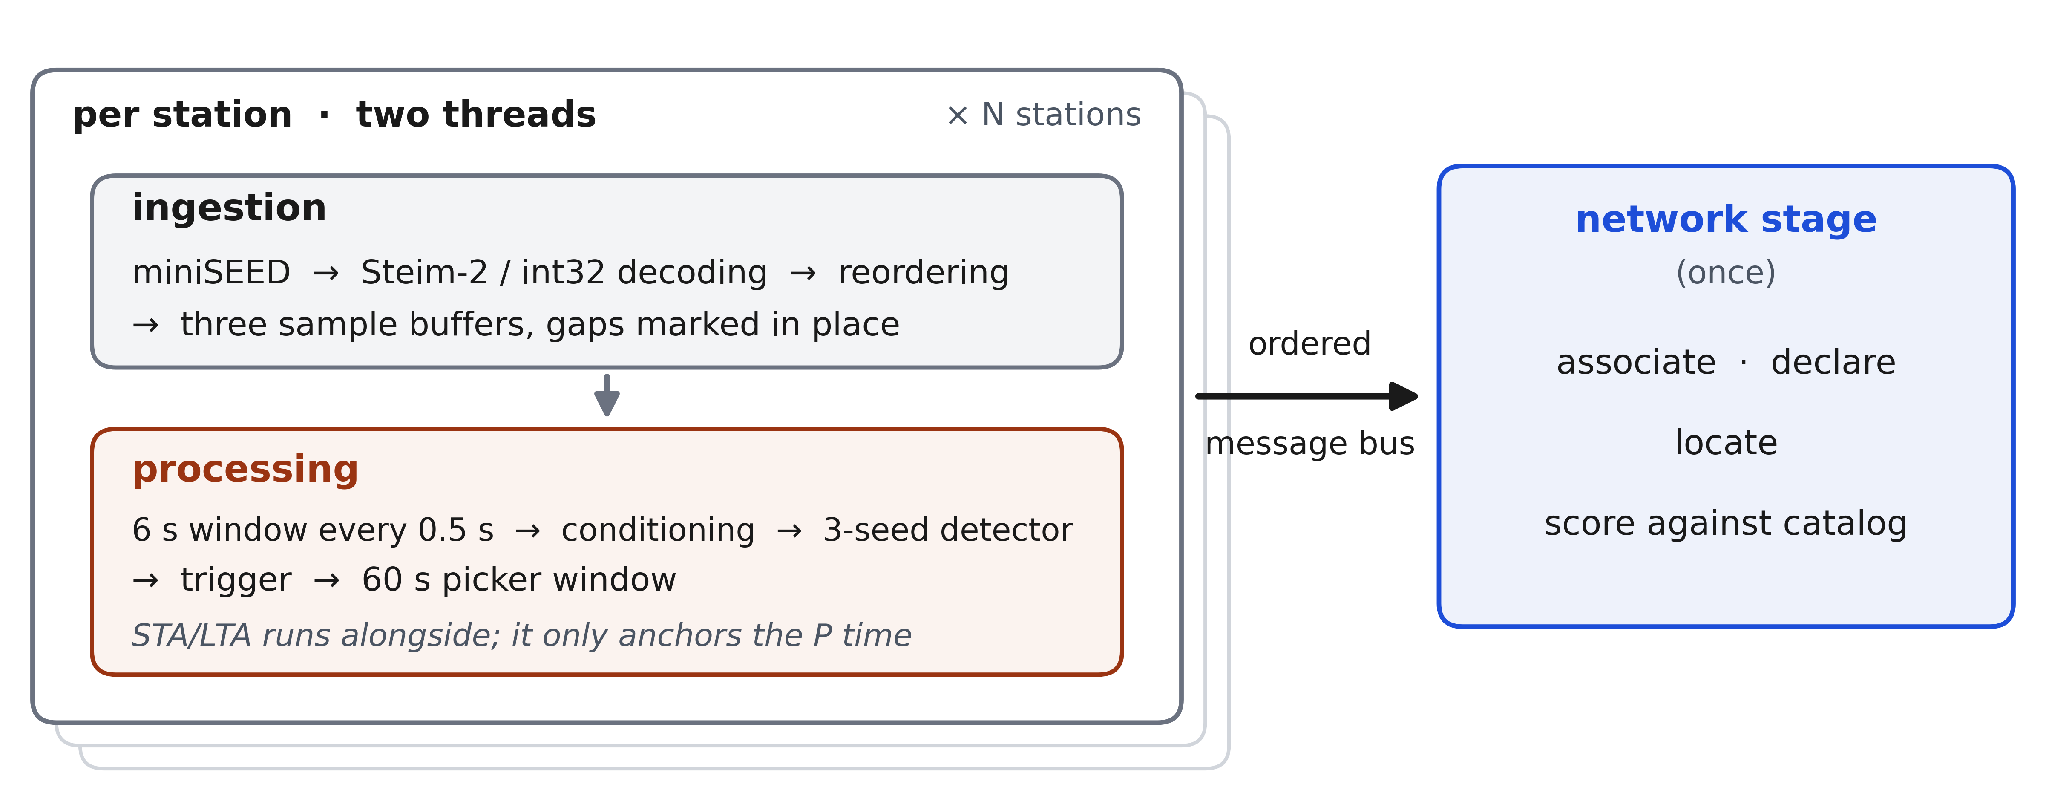
\includegraphics[width=\textwidth]{figures/fig1_pipeline.png}
  \caption{Architecture of the real-time pipeline. Each station runs an ingestion and a
    processing thread; a network stage associates station detections, declares and
    locates events and scores them against a catalog. The recursive \stalta{} never
    triggers; it only supplies the reported P time of a learned trigger.}\label{fig:pipeline}
\end{figure}

\begin{figure}
  \centering
  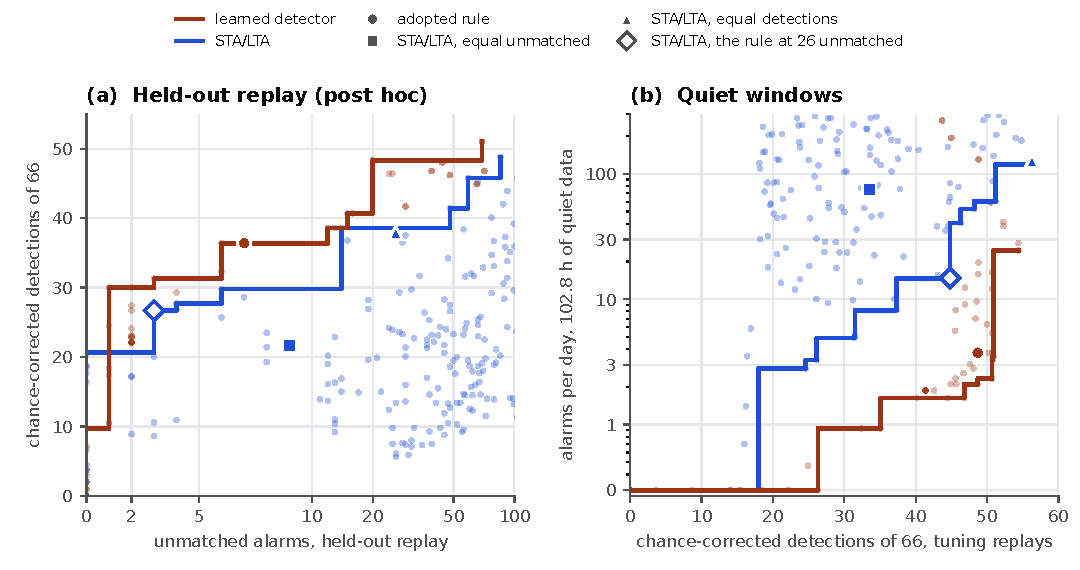
\includegraphics[width=\textwidth]{figures/fig7_operating_curves.pdf}
  \caption{Every trigger setting of both detectors (60 of the learned detector, and the 216 of
    \stalta{}'s 648 that have the re-arm ratio of 1.5 at which it was fixed,
    Section~S18; dots), with each detector's envelope (lines) and the selected
    settings (markers). (a)~Held-out replay, post hoc: chance-corrected detections against
    unmatched alarms. (b)~Alarms per day on 102.8~h of quiet data against
    chance-corrected detections on the tuning replays; settings without an alarm are
    drawn on the bottom edge. Open diamond: the \stalta{} setting that the
    equal-unmatched rule selects when applied to 26 rather than 25 unmatched alarms
    (Section~S16).}\label{fig:curves}
\end{figure}

\subsection{Learned detector versus STA/LTA}\label{sec:vs-stalta}

\stalta{} settings were tuned over 648 combinations, and two rules fixed before the
held-out run selected one setting at equal unmatched alarms (2--20~Hz, 1 and 30~s,
ratio 8, vertical) and one at equal detections (2--10~Hz, 0.5 and 10~s, ratio 6,
vertical). At comparable unmatched alarms (7 and 9), the learned detector detects
68\% more held-out events, with 36.4 against 21.7 chance-corrected detections, a
difference of 14.7 (95\% interval 5.9--23.7; 7.9--22.2 with 10-minute blocks; exact
McNemar $p = 0.003$). The difference lies in M2--4 events (12 against 4 of 27 M2--3
events and 21 against 14 of 32 M3--4 events), whereas \stalta{} detects all six
M4--5 events and the learned detector five. At comparable detections (37.9 against
36.4), \stalta{} raises about three times the unmatched alarms, 26 against 7 held out
and 63 against 26 on the tuning data (Table~\ref{tab:detectors}, Section~S18).
\stalta{} alarms 1.0--1.3~s earlier on the two largest events, because it triggers on
the onset sample whereas the window detector must see the P wave inside a 6~s window;
the taper and the filter applied within each window also down-weight its newest
samples, which may add to the delay.

\subsection{Other detectors and a second held-out sequence}\label{sec:others}

EQTransformer and PhaseNet were run through SeisBench 0.12.6 in place of the
detector, each 6~s window receiving the largest model output within it, with
everything downstream unchanged. In the \emph{causal} mode the model input ends at the
end of the window, as in real-time operation, and in the \emph{look-ahead} mode it is
centered on the window, which gives an offline upper bound. For each model and for
FilterPicker, the weights and trigger setting were selected on the tuning replays by
the two rules above, and both rules chose the INSTANCE weights \citep{michelini2021}
for the published models. The Simav sequence was replayed once with every setting
frozen, on the six archive stations within 300~km, against 56 cataloged events, 39 of
them below M2 (Table~\ref{tab:detectors}, Figure~\ref{fig:detectors}).

\begin{table}[pos=htbp]
  \centering\footnotesize
  \caption{Every detector at the settings selected on the tuning data: the two held-out
  sequences, the quiet windows and the public KOERI event sets.}\label{tab:detectors}
  \setlength{\tabcolsep}{2.6pt}
  \begin{tabular}{@{}lcccccccc@{}}
    \toprule
    & \multicolumn{3}{c}{S\i{}nd\i{}rg\i{} \Mw{}~6.1 (66)} & \multicolumn{3}{c}{Simav \Mw{}~4.8 (56)} & Quiet & KO (46) \\
    \cmidrule(lr){2-4}\cmidrule(lr){5-7}\cmidrule(lr){8-8}\cmidrule(lr){9-9}
    Detector, rule & Corr. & Unm. & Difference & Corr. & Unm. & Difference & per day & Det./Unm. \\
    \midrule
    learned                       & 36.4 & 7  &                       & 35.1 & 17 &                      & 3.7   & 36/25 \\
    \stalta{}, equal unm.         & 21.7 & 9  & $+14.7$ (5.9, 23.7)   & 29.1 & 14 & $+6.0$ ($-2.4$, 14.3) & 75.4  & 23/5 \\
    \stalta{}, equal det.         & 37.9 & 26 & $-1.5$ ($-9.7$, 6.6)  & 40.9 & 41 & $-5.8$ ($-12.5$, 0.8) & 127.0 & 39/17 \\
    FilterPicker, equal unm.      & 28.8 & 8  & $+7.6$ (1.4, 14.1)    & 33.8 & 18 & $+1.3$ ($-7.4$, 9.8)  & 82.4  & 31/12 \\
    FilterPicker, equal det.      & 34.9 & 16 & $+1.5$ ($-5.6$, 8.7)  & 39.0 & 49 & $-3.9$ ($-12.7$, 4.7) & 207.1 & 36/32 \\
    PhaseNet, both                & 33.3 & 12 & $+3.1$ ($-4.0$, 10.5) & 36.8 & 28 & $-1.8$ ($-8.2$, 4.1)  & 3.5   & 32/15 \\
    EQTransformer, equal unm.     & 11.0 & 13 & $+25.5$ (15.3, 35.4)  & 22.7 & 15 & $+12.4$ (2.9, 21.5)  & 1.6   & 24/16 \\
    EQTransformer, equal det.     & 34.0 & 50 & $+2.4$ ($-9.1$, 13.9) & 32.3 & 55 & $+2.8$ ($-5.5$, 11.1) & 6.1   & 34/37 \\
    \addlinespace
    \multicolumn{9}{@{}l}{\emph{Look-ahead, offline only}} \\
    PhaseNet, equal unm.          & 42.8 & 23 & $-6.4$ ($-15.4$, 2.3) & 41.2 & 35 & $-6.1$ ($-13.5$, 1.0) & 7.2   & 38/23 \\
    PhaseNet, equal det.          & 38.8 & 9  & $-2.3$ ($-9.2$, 4.3)  & 41.4 & 27 & $-6.3$ ($-13.1$, 0.3) & 3.3   & 32/14 \\
    EQTransformer, both           & 32.2 & 11 & $+4.2$ ($-6.7$, 15.3) & 33.4 & 25 & $+1.7$ ($-6.2$, 9.7)  & 2.6   & 35/15 \\
    \bottomrule
  \end{tabular}
  \tablenote{Corr.: chance-corrected detections; Unm.: unmatched alarms; difference:
    learned detector's chance-corrected detections minus other's, with 95\% paired
    bootstrap interval by events. Quiet: alarms per day on 102.8~h of AFAD quiet
    windows. KO: detected events and unmatched alarms on demo\_ko and marmara\_ko
    together. Settings: \stalta{} as in Section~\ref{sec:vs-stalta}; FilterPicker
    windows 6/10/0.4~s with thresholds 15 and 10 (equal unm.) and 3/5/0.2~s with 4 and
    10 (equal det.); published models with INSTANCE weights at threshold $\times$
    windows $0.7\times2$ (PhaseNet), $0.8\times2$ and $0.3\times8$ (EQTransformer),
    and with look-ahead $0.4\times8$, $0.6\times8$ (PhaseNet) and $0.5\times8$
  (EQTransformer).}
\end{table}

\begin{figure}
  \centering
  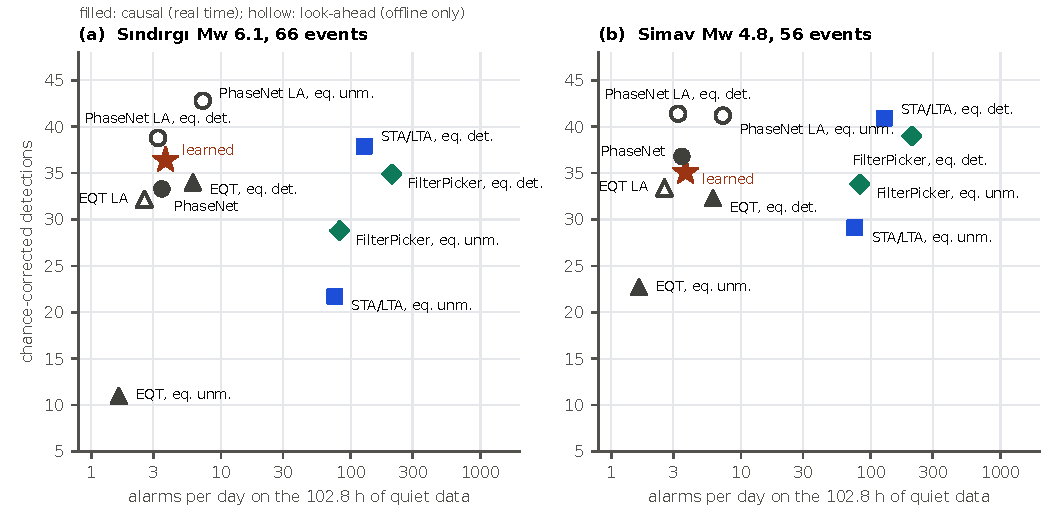
\includegraphics[width=\textwidth]{figures/fig3_detectors.pdf}
  \caption{Every detector of Table~\ref{tab:detectors}: chance-corrected detections on
    each held-out sequence against alarms per day on 102.8~h of quiet data
    (logarithmic). Up and to the left is better. Filled markers run in real time; hollow markers use
    input past the window and cannot.}\label{fig:detectors}
\end{figure}

On Simav the direction of the \stalta{} comparison repeats, but not its size. At
comparable unmatched alarms (17 and 14) the learned detector detected 35.1
chance-corrected events against 29.1, a difference of 6.0 whose interval includes
zero, and the gain again lies in M2--4 events. Most of Simav's events are below M2, the lower limit of the detector's training
events, where no detector separates reliably from noise. Pooled over both sequences, with the
chance correction and bootstrap within each, the difference is 20.7 (8.8--32.8; exact
McNemar $p = 0.001$), a summary that neither protocol specified.

The gain over \stalta{} is not specific to the pipeline's detector. Causal PhaseNet
matched it on both sequences (pooled difference 1.4, $-8.1$ to 11.0), with 12 and 28
unmatched alarms against 7 and 17 and with 15 quiet-window alarms against 16, whereas
causal EQTransformer was not competitive at equal unmatched alarms. With look-ahead,
PhaseNet detected the most events of any detector, but only offline and at three times
the unmatched alarms and twice the quiet-window rate of the learned detector (7.2
against 3.7 per day, exact $p = 0.04$). This gap does not come from scoring the
window at the edge of the model input. Under a protocol committed before any of its
scores, ending the input 1 or 2~s after the window left PhaseNet level with the
learned detector and EQTransformer far below it (Section~S15). FilterPicker is the
strongest classical detector tested. At equal unmatched alarms it detected fewer
held-out events than the learned detector (difference 7.6, 1.4 to 14.1; McNemar
$p = 0.021$) and as many on Simav, and at equal detections it matched the learned
detector with two to three times its unmatched alarms. On the quiet windows, however,
its two settings raised 82.4 and 207.1 alarms per day, 22 and 55 times the learned
detector's rate, mostly at two stations, CMH and KIRK.

\subsection{False alarms on quiet data}\label{sec:quiet}

Over 102.8~h without a cataloged event within 250~km, the learned detector raised 16
alarms, 3.74 per day (95\% interval 2.14--6.07), against 323, 75.4 per day
(67.4--84.1), for \stalta{} at equal unmatched alarms (rate ratio 0.050,
0.028--0.082). That ratio of about 20 belongs to the two selected settings, because
\stalta{} was matched on unmatched rather than false alarms. Over the full grids
(Figure~\ref{fig:curves}b), at equal tuning detections, the quietest \stalta{}
setting raises 5 to 29 times the alarms of the quietest learned setting (4.9 against
  0.93 per day at 30 chance-corrected detections, 14.7 against 1.63 at 44 and 60.5
against 2.1 at 48.7). The rate of \stalta{} is similar in the held-out event window (72
per day) and on quiet data, whereas the learned detector's falls from 56 to 3.7 per
day, which suggests that most of its unmatched alarms in the event windows were
uncataloged aftershocks. On 5.8~h of public KOERI quiet data the learned detector
raised 1 alarm against 25 for \stalta{}.

\begin{table}[pos=htbp]
  \centering\small
  \caption{Alarms of the learned detector on the AFAD quiet windows (102.8~h), by criteria
    that need no judgment of the waveforms.}\label{tab:quietclass}
  \begin{tabular}{@{}lcl@{}}
    \toprule
    Class & Alarms & Criterion \\
    \midrule
    KIRK's instrumental pulse & 9 & KIRK declared; its detection in pulse slot \\
    seismic, picker-confirmed & 4 & S$-$P test with PhaseNet or EQTransformer picks \\
    undetermined & 3 & neither \\
    \midrule
    all alarms & 16 & 3.74 (2.14--6.07) per day \\
    excluding picker-confirmed & 12 & 2.80 (1.45--4.89) per day \\
    KIRK's pulse only & 9 & 2.10 (0.96--3.99) per day \\
    \midrule
    \multicolumn{3}{@{}l}{\emph{Sensitivity: picker rule on any associated pair of stations}} \\
    pulse / seismic / undetermined & 8 / 5 / 3 & alarm~1 confirmed through BAND--CMH \\
    excluding picker-confirmed & 11 & 2.57 (1.28--4.60) per day \\
    \bottomrule
  \end{tabular}
  \tablenote{Upper rows: classification committed before it was run; last two rows: same picker rule
    on every pair of stations associated with an alarm, also specified before it was
    run. Rates: alarms per day with exact Poisson 95\% intervals. Each alarm is listed
  in Table~S11.}
\end{table}

The 16 alarms were classified by criteria that need no judgment of the waveforms
(Table~\ref{tab:quietclass}). Nine were declared with KIRK, whose detection fell
58.6--58.8~s after a 10-minute mark, the slot of a periodic instrumental pulse.
Detections associate within the P travel time between their stations plus 3~s, 14 to
67~s for the pairs with KIRK, so a faulty station raises the network's alarm rate
through chance coincidences with the other stations' triggers. A rule
fixed before it was run confirms a seismic source when a published picker finds P and
S at two declaring stations and the two S$-$P distances fit the station separation
and the P-time difference. It confirms four alarms of the learned detector, one an
M2.4 listed by the European-Mediterranean Seismological Centre but not by AFAD, and
three of the 323 \stalta{} alarms, all among the same events. Without them the rates
are 2.80 and 74.7 per day, and under a classification that is the same for both
detectors the contrast is unchanged. KIRK's pulse, confined to May--June 2024 and
absent from the event replays, is a single 0.3~s pulse locked to UTC
(Figure~\ref{fig:quietexamples}), and without KIRK the learned detector's rate would be 1.40 per day, a figure that
also removes alarm~15, a picker-confirmed earthquake declared with KIRK outside the
pulse slot (Table~S11). Of the 323 \stalta{} alarms, 263 rest on signals shorter than 3~s at both
stations, most of them spikes under 0.5~s, such as the isolated spikes at CMH that
the learned detector ignores.

\begin{figure}
  \centering
  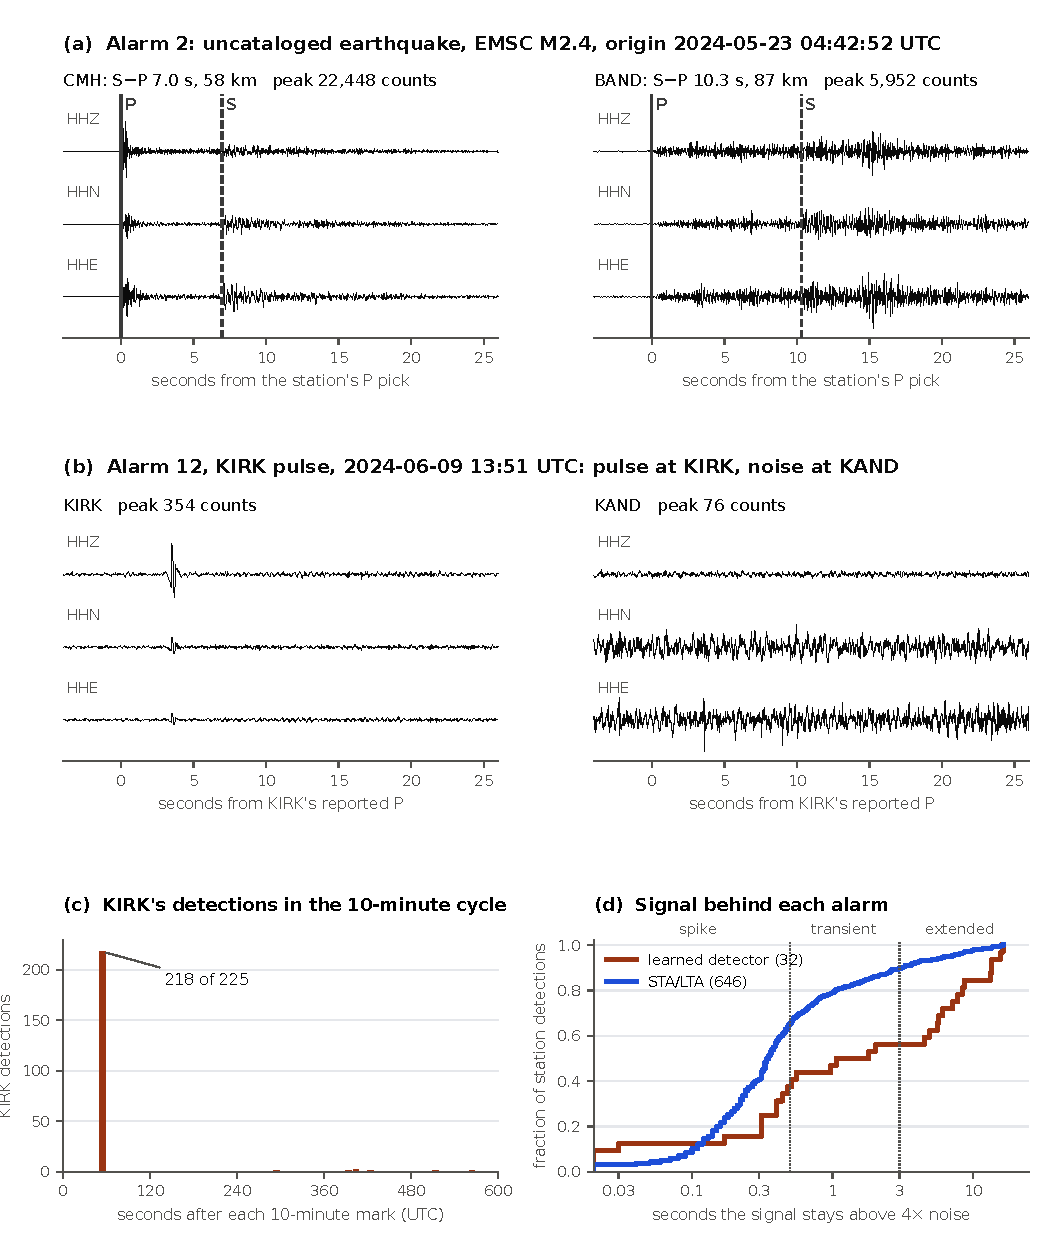
\includegraphics[width=\textwidth]{figures/fig6_quiet_alarms.pdf}
  \caption{Alarms of the learned detector on the AFAD quiet windows. (a)~Alarm~2, an
    uncataloged earthquake (M2.4 in the EMSC catalog; origin time from EMSC) recorded at
    both declaring stations, with the pipeline's P (solid) and S (dashed) picks.
    (b)~Alarm~12: KIRK's instrumental pulse, about 0.3~s without S wave or coda,
    coinciding with background noise at KAND. Records band-passed 1--20~Hz.
    (c)~KIRK's 225 detections by time after each 10-minute mark in UTC (10~s bins).
    (d)~Duration of the signal behind each alarm at each declaring station, as the
    time its envelope stays above four times the noise of the preceding 25~s, for the
    learned detector's 16 alarms and \stalta{}'s 323.}\label{fig:quietexamples}
\end{figure}

\subsection{Alert latency}\label{sec:latency}

For the Marmara \Mw{}~6.2, the alarm came 11.0~s after origin, and the S wave reached
station ELBA (38~km) 2.1~s later. Because the alarm carries no magnitude or shaking
estimate, such margins bound the lead time a warning could have had. Because
stations are processed independently, a recorded replay can be re-run through the
network stage for every subset of stations. Over every subset that declared the
\Mw{}~6.2, the alert exceeds the P travel time to the second-nearest station by a
median of 2.05~s (interquartile range 0.6--2.8~s), and two stations alone, ARNA and
ELBA, give the same alert as all eight (Sections~S5--S7).

\subsection{Detector ranking on a continuous record}\label{sec:ranking}

Six detectors were scored on a continuous 728-day record at station MANT: the
pipeline's learned detector and \stalta{}, and four offline detectors, a classical
\stalta{} \citep{allen1978}, two P-wave detectors that score 3.4~s windows and differ
only in their noise windows, and a 6~s detector with station scaling
(Table~\ref{tab:roc}, Figure~\ref{fig:recall}). The pipeline's two detectors are almost
indistinguishable by event AUC (0.9910 for \stalta{}, 0.9892 for the learned
detector; difference 0.0016, 0.0000--0.0035), yet at one window false alarm per day the learned detector finds 34.8\% of the events against 22.2\%, 1.6 times as many. Among
the offline detectors, recall at one window false alarm per day is in the exact reverse
order of event AUC. Because all six are scored on the same record, the inversion is a
property of the metric, which integrates over all false positive rates whereas
operation uses rates of order $10^{-4}$. The guard over which an event is scored
extends 60~s past P, so that every detector can also score the S wave. Scored only
from windows that end at least 1~s before the predicted S, over the 12\,206 events with
S$-$P of at least 7~s, the inversion at one window false alarm per day remains (33.8\%
against 21.4\%), although \stalta{} then draws level or ahead at ten per day
(Section~S14).

\begin{table}[pos=htbp]
  \centering\small
  \caption{Recall of 13\,056 events with SNR~$\geq 3$ over 728 days at MANT at three alarm
    budgets (window false alarms per day at the one station, Section~\ref{sec:protocols}).}\label{tab:roc}
  \begin{tabular}{@{}lcccc@{}}
    \toprule
    Detector & Event AUC & 100/day & 10/day & 1/day \\
    \midrule
    \multicolumn{5}{@{}l}{\emph{Run by the pipeline}} \\
    \stalta{} (causal, 2--20~Hz) & 0.9910 & 0.991 & 0.730 & 0.222 \\
    6~s detector (per-window)    & 0.9892 & 0.979 & 0.743 & 0.348 \\
    \addlinespace
    \multicolumn{5}{@{}l}{\emph{Offline}} \\
    \stalta{} (classical)       & 0.9795 & 0.928 & 0.548 & 0.132 \\
    P-wave, amplitude-matched   & 0.9622 & 0.903 & 0.627 & 0.183 \\
    P-wave, natural negatives   & 0.9516 & 0.861 & 0.573 & 0.219 \\
    6~s detector (station scaling) & 0.9403 & 0.864 & 0.741 & 0.316 \\
    \bottomrule
  \end{tabular}
  \tablenote{Event AUC: maximum score within each event's guard window against maximum
    score over random stretches of equal length, away from cataloged events, of same
  record.}
\end{table}

\begin{figure}
  \centering
  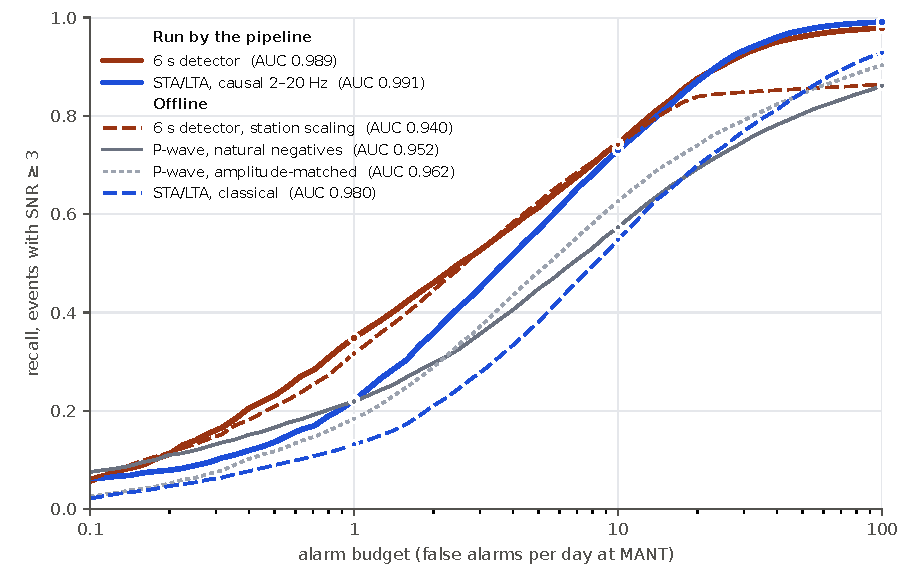
\includegraphics[width=0.85\textwidth]{figures/fig5_recall_budget.pdf}
  \caption{Recall of the six detectors of Table~\ref{tab:roc} against the alarm budget
    (window false alarms per day), 20 budgets a decade; dots mark the budgets of the
    table. Solid wide lines: detectors run by the pipeline; dashed: their offline
    counterparts.}\label{fig:recall}
\end{figure}

% ---------------------------------------------------------------------------
\section{Discussion}\label{sec:discussion}

A detector for early warning is best evaluated at the operating point at which it
will be used and on the data it will see. Matched on unmatched alarms and replayed on
quiet data, the learned detector and the classical triggers separate clearly, whereas
event-level ROC-AUC barely separates the pipeline's two detectors and ranks four
offline ones in the reverse order of their recall.

The classical detectors are neither obsolete nor superior. The learned detector gains
in M2--4 events that an amplitude criterion cannot separate from noise, and it keeps
that sensitivity at a small fraction of the classical detectors' alarm rate on quiet
data. The classical detectors, however, alarm 1.0--1.3~s earlier on the largest
events, cost orders of magnitude less, as measured for \stalta{}, and time the onset to
a sample, which is why the pipeline uses \stalta{} for timing rather than for
decisions. Causal PhaseNet, trained on another country's data, matched the learned
detector, and no published model that can run in real time was shown to exceed it at
an alarm rate matched on the tuning data. The gain thus comes from learned detection
rather than from this particular detector, and what distinguishes the pipeline's
detector is that it reaches this level in a self-contained program with 142\,059
parameters per network.

The computational design carries much of the protocol's weight. Cached window
probabilities and deterministic replays made trigger grids of hundreds of settings,
seven scoring passes per setting and evaluations committed in advance practical, and
replaying every station subset separated the geometric term of the alert time from
the terms the detector controls. The P travel time to the second station dominates
the alert, and the detector contributes about 2~s after it, so that stations near
source regions shorten the alert more than a faster detector would. Two failures of
the data path were found only by complete replays (Section~S2). The dataloggers
nearest the \Mw{}~6.2 switched to uncompressed integers, which a decoder that accepted
only Steim-2 silently rejected, and an earlier version that dropped samples under load
shifted later samples in time and lost 15 of 44 detections.

\subsection{Limitations}\label{sec:limits}

The study rests on one regional network and two held-out sequences, the second with
an advantage over \stalta{} that was not significant, and the first scored repeatedly
for post hoc analyses. The ranking on a continuous record rests on one station. The catalog is incomplete for small events, so that unmatched alarms only bound false
alarms, and absorbing detections within 40~s as coda trades the resolution of closely
spaced events, a doublet among them, for fewer false alarms in dense sequences, and the quiet-window classes use no analyst picks. The published models ran
with pre-trained weights and the pipeline's trigger rule, and fine-tuning them on the
detector's training split might improve them. The input is a replay of archived
files, and a live SeedLink client, with its latency, packet loss and clock problems,
is not implemented. Further held-out sequences committed before extraction, more
stations and a live shadow run beside AFAD's alerts would address these limits.

% ---------------------------------------------------------------------------
\section{Conclusions}\label{sec:conclusions}

A self-contained, verified real-time pipeline and a replay protocol with chance
correction and held-out sequences with protocols committed in advance measure
seismic detectors at their
operating point. Under this protocol, a learned detector found 36.4 chance-corrected
events of 66 against 21.7 for \stalta{} at comparable unmatched alarms on one held-out
sequence and 35.1 of 56 against 29.1, within the uncertainty, on a second. On quiet
data it raised a small fraction of the classical detectors' alarms, and causal
PhaseNet matched it. Two detectors with nearly equal event AUC differed by a factor of
1.6 in recall at one window false alarm per day, and detectors for early warning are
therefore best compared on continuous records at fixed alarm budgets.

% ---------------------------------------------------------------------------
\printcredits

\section*{Code availability}

Name of the software: ayzek. Developer: H. O\u{g}uz Bolat
(\href{mailto:oguz.bolat@std.yildiz.edu.tr}{oguz.bolat@std.yildiz.edu.tr}), first
available in 2026. Program language: C++23, with Python tools for model export and
evaluation. Hardware requirements: an x86-64 or aarch64 processor; tested on a desktop
computer and on a Raspberry Pi~4. Software required: Meson and Ninja and a C++23
compiler (GCC~16 or Clang); no machine-learning runtime. Program size: about 9\,400
lines of C++ and 6.5~MB of model weights. License: GNU General Public License,
version~3 or later. The source code, model weights, documentation and the scripts that
reproduce every result (\texttt{tools/reproduce\_all.sh}, with expected values in
\texttt{bench/claims.json}) are available at \url{https://github.com/hogib/ayzek}
(release v0.1.0-beta.6), archived at \url{https://doi.org/10.5281/zenodo.23672495}. The FilterPicker port is
derived from the C code of \citet{lomax2012} (GNU GPL version~2 or later). Software
versions are listed in Table~S9.

\section*{Data availability}

Waveforms are from the Turkish National Seismic Network \citep{afad1990}, obtained
through the AFAD archive service, and from the KO network of KOERI \citep{koeri1971}
through its FDSN service; the AFAD and KOERI catalogs are public. The AFAD waveforms
cannot be redistributed. The three KOERI datasets of Table~\ref{tab:replays}, which
reproduce the principal results, are attached to the pipeline's release. The offline
evaluation code is available at \url{https://github.com/SismoKaos-Research/cnn_earthquake},
the training code of the detector at \url{https://github.com/hogib/cascade} and that of
the picker at \url{https://github.com/hogib/sphase}.

\section*{Declaration of competing interests}

The authors declare that they have no known competing financial interests or personal
relationships that could have appeared to influence the work reported in this paper.

\section*{Funding}

This research did not receive any specific grant from funding agencies in the public,
commercial, or not-for-profit sectors.

\section*{Acknowledgments}

The authors thank AFAD and KOERI for access to their waveform data and earthquake
catalogs.

\section*{Declaration of generative AI and AI-assisted technologies in the manuscript preparation process}

During the preparation of this work the authors used Claude Opus~5 and Claude
Opus~5.5 (Anthropic) to develop and refactor parts of the pipeline code, extend the
analysis and edit the manuscript text. After using these tools, the authors reviewed
and edited the content as needed and take full responsibility for the content of the
published article.

\bibliographystyle{cas-model2-names}
\bibliography{refs}

\end{document}
